\chapter{क्रिस्टल II: आयनिक, सहसंयोजी और आण्विक ठोस}\label{ch:b1:crystals-ionic-covalent}

कुचला हुआ खाने का नमक छोटे-छोटे घनों में टूटता है; हीरा सबसे कठोर
प्राकृतिक पदार्थ है, फिर भी उन्हीं कार्बन परमाणुओं से बना ग्रेफ़ाइट इतना नरम है
कि उससे लिखा जा सके; बर्फ़ पानी पर तैरती है। ये सब \omterm{def:b1:crystals-metals:crystal}{क्रिस्टल} हैं, पर इनके
कण अलग-अलग तरीकों से जुड़े रहते हैं: आयन स्थिरवैद्युत
आकर्षण से, परमाणु \omterm{def:b1:lewis-resonance-vsepr:lewis}{सहसंयोजी आबंधों} से, अणु \cref{ch:b1:intermolecular-forces-solvents}
के अंतराआण्विक बलों से। यह अध्याय
पिछले अध्याय की कोष्ठिका-ज्यामिति को ठोसों के इन तीन परिवारों पर लागू करता है,
और आयनों के आकारों से समझाता है कि सोडियम क्लोराइड
और सीज़ियम क्लोराइड भिन्न संरचनाएँ क्यों अपनाते हैं।

\begin{recall}
कोष्ठिका की \omterm{def:b1:crystals-metals:multiplicity}{बहुकता}, \omterm{def:b1:crystals-metals:coordination}{उपसहसंयोजन संख्या} और \omterm{def:b1:crystals-metals:compactness}{संहतता}, तथा
\omterm{def:b1:crystals-metals:packings}{फलक-केंद्रित घनीय} \omterm{def:b1:crystals-metals:lattice}{जालक} के अष्टफलकीय और \omterm{def:b1:crystals-metals:site}{चतुष्फलकीय स्थल}
\cref{ch:b1:crystals-metals} में परिभाषित किए गए; \omterm{def:b1:crystals-metals:crystal}{क्रिस्टल} का घनत्व
$\rho = ZM/(N_A V)$ है (\cref{prop:b1:crystals-metals:density})। \omterm{def:b1:periodicity:radius}{आयनिक त्रिज्याओं} का
परिचय \cref{def:b1:periodicity:radius} में दिया गया।
\end{recall}

\section{आयनिक क्रिस्टल और त्रिज्या अनुपात}

\begin{definition}[आयनिक क्रिस्टल]\label{def:b1:crystals-ionic-covalent:ionic-crystal}
\emph{आयनिक क्रिस्टल}\index{आयनिक क्रिस्टल} धनायनों और
ऋणायनों का \omterm{def:b1:crystals-metals:crystal}{क्रिस्टल} है जिन्हें स्थिरवैद्युत आकर्षण जोड़े रखता है। हर आयन विपरीत आवेश
वाले आयनों से घिरा होता है; \omterm{def:b1:crystals-metals:crystal}{क्रिस्टल} विद्युत रूप से उदासीन है, इसलिए
किसी कोष्ठिका में धनायनों और ऋणायनों की संख्याओं का अनुपात सूत्र वाला होता है।
\end{definition}

\begin{proposition}[आयनिक क्रिस्टलों के गुण]\label{prop:b1:crystals-ionic-covalent:ionic-properties}
\omterm{def:b1:crystals-ionic-covalent:ionic-crystal}{आयनिक क्रिस्टल} कठोर पर भंगुर होते हैं (एक परत के खिसकने से समान चिह्न वाले आयन
आमने-सामने आ जाते हैं, और \omterm{def:b1:crystals-metals:crystal}{क्रिस्टल} विदलित हो जाता है), उनके गलनांक
ऊँचे होते हैं, ठोस अवस्था में वे चालन नहीं करते पर पिघलने या घुलने पर करते हैं,
और उच्च परावैद्युतांक वाले \omterm{def:b1:intermolecular-forces-solvents:solvent-classes}{ध्रुवीय विलायकों} में घुलते हैं।
\end{proposition}
\admitted

\begin{definition}[त्रिज्या अनुपात]\label{def:b1:crystals-ionic-covalent:radius-ratio}
त्रिज्या $r_+$ वाले धनायन और त्रिज्या
$r_-$ वाले ऋणायन के \omterm{def:b1:crystals-ionic-covalent:ionic-crystal}{आयनिक क्रिस्टल} में \emph{त्रिज्या अनुपात}\index{त्रिज्या अनुपात} $x = r_+/r_-$ है
(प्रायः $x < 1$, क्योंकि धनायन ऋणायनों से छोटे होते हैं)।
\end{definition}

\begin{proposition}[त्रिज्या-अनुपात नियम]\label{prop:b1:crystals-ionic-covalent:rule}
कठोर-गोला मॉडल में, ऐसी संरचना जिसमें हर धनायन $n$
ऋणायनों को छूता है, केवल तभी स्थायी है जब ऋणायन एक-दूसरे को न छुएँ, जिसके लिए
आवश्यक है कि $x$ ज्यामिति द्वारा तय एक सीमा से ऊपर हो: $x \ge \sqrt3 - 1
\approx 0.732$, 8 पड़ोसियों (घन) के लिए; $x \ge \sqrt2 - 1 \approx 0.414$,
6 (अष्टफलक) के लिए; $x \ge \sqrt{3/2} - 1 \approx 0.225$, 4
(चतुष्फलक) के लिए। अपनाई जाने वाली संरचना वह है जिसकी \omterm{def:b1:crystals-metals:coordination}{उपसहसंयोजन संख्या}
$x$ द्वारा अनुमत संख्याओं में सबसे अधिक हो।
\end{proposition}

\begin{proof}
धनायन अपने संपर्क में स्थित $n$ ऋणायनों के बीच के रिक्त स्थान में बैठता है। सीमा पर
ऋणायन एक-दूसरे को भी छूते हैं। घन: ऋणायन कोर $2r_-$ वाले घन के
कोनों पर हैं और धनायन उसके केंद्र पर, इसलिए $r_+ +
r_- = \sqrt3\,r_-$। अष्टफलक: भुजा $2r_-$ वाले वर्ग में चार ऋणायन,
उसके केंद्र पर धनायन, $r_+ + r_- = \sqrt2\,r_-$। चतुष्फलक:
ऋणायन कोर $\sqrt2\,r_-$ वाले घन के एकांतर कोनों पर, धनायन
केंद्र पर, $r_+ + r_- = \frac{\sqrt3}{2}\sqrt2\,r_- = \sqrt{3/2}\,r_-$।
$r_-$ से भाग देने पर सीमाएँ मिलती हैं। सीमा से नीचे धनायन अपने लिए बहुत बड़े
रिक्त स्थान में खड़खड़ाता है: ऋणायन प्रतिकर्षित करते हैं पर आकर्षण
नहीं बढ़ता, इसलिए छोटे रिक्त स्थान वाली निम्नतर उपसहसंयोजन को वरीयता मिलती है।
\end{proof}

\begin{omfigure}
\begin{tikzpicture}[font=\small, >={Stealth}]
  \draw[->, thick] (0,0) -- (12.4,0) node[right] {$x = r_+/r_-$};
  \foreach \x/\l in {0/0, 2.7/0.225, 4.97/0.414, 8.78/0.732, 12/1} {
    \draw (\x,0.12) -- (\x,-0.12) node[below] {\l};
  }
  \fill[omDef!15] (2.7,0.2) rectangle (4.97,1.0);
  \fill[omProp!15] (4.97,0.2) rectangle (8.78,1.0);
  \fill[omThm!15] (8.78,0.2) rectangle (12,1.0);
  \node[align=center] at (3.83,0.6) {4: ZnS};
  \node[align=center] at (6.87,0.6) {6: NaCl};
  \node[align=center] at (10.4,0.6) {8: CsCl};
  \foreach \x/\l in {3.91/\ce{ZnS}, 6.76/\ce{NaCl}, 10.08/\ce{RbCl}, 11.54/\ce{CsCl}} {
    \draw[omExo, thick] (\x,-0.55) -- (\x,-0.95);
    \node[below, omExo] at (\x,-0.95) {\l};
  }
\end{tikzpicture}

{\small त्रिज्या-अनुपात नियम: $x$ द्वारा अनुमत धनायन की \omterm{def:b1:crystals-metals:coordination}{उपसहसंयोजन
संख्या}, और चार लवणों के मापे गए अनुपात (शैनन त्रिज्याएँ)।
रुबिडियम क्लोराइड, 0.84 पर, \ce{CsCl} प्रकार का होना चाहिए पर
\ce{NaCl} प्रकार अपनाता है: नियम एक मार्गदर्शक है, कोई अटल नियम नहीं
(\cref{exo:b1:crystals-ionic-covalent:12})।}
% ledger: rion:Zn2+IV, rion:S2-VI, rion:Na+VI, rion:Cl-VI, rion:Rb+VI,
% rion:Cs+VIII
\end{omfigure}

\section{चार संरचना-प्रकार}

\begin{definition}[संरचना-प्रकार]\label{def:b1:crystals-ionic-covalent:structure-type}
\omterm{def:b1:crystals-ionic-covalent:ionic-crystal}{आयनिक क्रिस्टलों} को कुछ संरचना-प्रकारों में वर्गीकृत किया जाता है, जिनके नाम
किसी प्रतिनिधि यौगिक पर रखे गए हैं:
\begin{itemize}
  \item \emph{सीज़ियम क्लोराइड प्रकार}\index{सीज़ियम क्लोराइड प्रकार}: ऋणायन
        घन के कोनों पर, धनायन उसके केंद्र पर (8:8);
  \item \emph{सैंधव-लवण प्रकार}\index{सैंधव-लवण प्रकार} (सोडियम क्लोराइड
        प्रकार): ऋणायन FCC \omterm{def:b1:crystals-metals:lattice}{जालक} पर, धनायन उसके सभी \omterm{def:b1:crystals-metals:site}{अष्टफलकीय
        स्थलों} में (6:6);
  \item \emph{ज़िंक-ब्लेंड प्रकार}\index{ज़िंक-ब्लेंड प्रकार}: ऋणायन FCC
        \omterm{def:b1:crystals-metals:lattice}{जालक} पर, धनायन उसके आधे \omterm{def:b1:crystals-metals:site}{चतुष्फलकीय स्थलों} में, एकांतर क्रम से हर दूसरे
        स्थल में (4:4);
  \item \emph{फ़्लुओराइट प्रकार}\index{फ़्लुओराइट प्रकार}: धनायन FCC
        \omterm{def:b1:crystals-metals:lattice}{जालक} पर, ऋणायन उसके सभी \omterm{def:b1:crystals-metals:site}{चतुष्फलकीय स्थलों} में (8:4), सूत्र
        \ce{MX2}; \emph{प्रतिफ़्लुओराइट प्रकार}\index{प्रतिफ़्लुओराइट प्रकार} में
        भूमिकाएँ उलट जाती हैं (\ce{Li2O}, 4:8)।
\end{itemize}
संख्याओं का जोड़ा धनायन और ऋणायन की \omterm{def:b1:crystals-metals:coordination}{उपसहसंयोजन संख्याएँ}
बताता है।
\end{definition}

\begin{omfigure}
\tdplotsetmaincoords{60}{100}
\begin{tikzpicture}[tdplot_main_coords, font=\small]
  \pic {omcubeo={3}};
    \node[aX={green!55!black}{6.5mm}] at (0,0,0) {};
  \node[aX={violet!70}{3.8mm}] at (0,1.5,0) {};
  \node[aX={green!55!black}{6.5mm}] at (0,3,0) {};
  \node[aX={violet!70}{3.8mm}] at (0,0,1.5) {};
  \node[aX={green!55!black}{6.5mm}] at (0,1.5,1.5) {};
  \node[aX={violet!70}{3.8mm}] at (0,3,1.5) {};
  \node[aX={violet!70}{3.8mm}] at (1.5,0,0) {};
  \node[aX={green!55!black}{6.5mm}] at (0,0,3) {};
  \node[aX={green!55!black}{6.5mm}] at (1.5,1.5,0) {};
  \node[aX={violet!70}{3.8mm}] at (0,1.5,3) {};
  \node[aX={violet!70}{3.8mm}] at (1.5,3,0) {};
  \node[aX={green!55!black}{6.5mm}] at (0,3,3) {};
  \node[aX={green!55!black}{6.5mm}] at (1.5,0,1.5) {};
  \node[aX={violet!70}{3.8mm}] at (1.5,1.5,1.5) {};
  \node[aX={green!55!black}{6.5mm}] at (1.5,3,1.5) {};
  \node[aX={green!55!black}{6.5mm}] at (3,0,0) {};
  \node[aX={violet!70}{3.8mm}] at (1.5,0,3) {};
  \node[aX={violet!70}{3.8mm}] at (3,1.5,0) {};
  \node[aX={green!55!black}{6.5mm}] at (1.5,1.5,3) {};
  \node[aX={green!55!black}{6.5mm}] at (3,3,0) {};
  \node[aX={violet!70}{3.8mm}] at (1.5,3,3) {};
  \node[aX={violet!70}{3.8mm}] at (3,0,1.5) {};
  \node[aX={green!55!black}{6.5mm}] at (3,1.5,1.5) {};
  \node[aX={violet!70}{3.8mm}] at (3,3,1.5) {};
  \node[aX={green!55!black}{6.5mm}] at (3,0,3) {};
  \node[aX={violet!70}{3.8mm}] at (3,1.5,3) {};
  \node[aX={green!55!black}{6.5mm}] at (3,3,3) {};
  \node at (1.5,1.5,-1.75) {\ce{NaCl} (सैंधव लवण)};
\end{tikzpicture}
\hspace{1cm}
\begin{tikzpicture}[tdplot_main_coords, font=\small]
  \pic {omcubeo={3}};
    \node[aX={green!55!black}{6.5mm}] at (0,0,0) {};
  \node[aX={green!55!black}{6.5mm}] at (0,3,0) {};
  \node[aX={green!55!black}{6.5mm}] at (0,0,3) {};
  \node[aX={green!55!black}{6.5mm}] at (0,3,3) {};
  \node[aX={blue!60}{7mm}] at (1.5,1.5,1.5) {};
  \node[aX={green!55!black}{6.5mm}] at (3,0,0) {};
  \node[aX={green!55!black}{6.5mm}] at (3,3,0) {};
  \node[aX={green!55!black}{6.5mm}] at (3,0,3) {};
  \node[aX={green!55!black}{6.5mm}] at (3,3,3) {};
  \node at (1.5,1.5,-1.75) {\ce{CsCl}};
\end{tikzpicture}

{\small बाएँ: सैंधव-लवण कोष्ठिका, \ce{Cl-} (हरा) FCC \omterm{def:b1:crystals-metals:lattice}{जालक} पर,
\ce{Na+} (बैंगनी) हर \omterm{def:b1:crystals-metals:site}{अष्टफलकीय स्थल} में। दाएँ: सीज़ियम क्लोराइड
कोष्ठिका, \ce{Cl-} कोनों पर, \ce{Cs+} (नीला) केंद्र पर। आयन संपर्क-आकार से
छोटे बनाए गए हैं।}
\end{omfigure}

\begin{proposition}[सैंधव-लवण और सीज़ियम क्लोराइड प्रकार]\label{prop:b1:crystals-ionic-covalent:nacl-cscl}
\omterm{def:b1:crystals-ionic-covalent:structure-type}{सैंधव-लवण प्रकार} में प्रति कोष्ठिका $Z = 4$ सूत्र इकाइयाँ होती हैं, आयन
कोर के अनुदिश छूते हैं, $a = 2(r_+ + r_-)$, और संरचना के लिए $\sqrt2 - 1
\le x$ आवश्यक है। \omterm{def:b1:crystals-ionic-covalent:structure-type}{सीज़ियम क्लोराइड प्रकार} में $Z = 1$, आयन
मुख्य विकर्ण के अनुदिश छूते हैं, $a\sqrt3 = 2(r_+ + r_-)$, और संरचना के लिए
$x \ge \sqrt3 - 1$ आवश्यक है।
\end{proposition}

\begin{proof}
सैंधव लवण: FCC \omterm{def:b1:crystals-metals:lattice}{जालक} के ऋणायन $4$ गिने जाते हैं, 4
\omterm{def:b1:crystals-metals:site}{अष्टफलकीय स्थलों} के धनायन $1 + 12 \times \frac14 = 4$। कोर के अनुदिश ऋणायन,
धनायन और ऋणायन एक के बाद एक संपर्क में हैं। ऋणायन एक-दूसरे पर नहीं चढ़ते
यदि फलक-विकर्ण, जिस पर तीन ऋणायन हैं जिनमें से अधिक-से-अधिक दो छूते हैं,
$a\sqrt2 \ge 4r_-$ को संतुष्ट करे, अर्थात् $2(r_+ + r_-)\sqrt2 \ge
4r_-$, या $x \ge \sqrt2 - 1$। सीज़ियम क्लोराइड: $8 \times \frac18 = 1$
ऋणायन और 1 धनायन; मुख्य विकर्ण पर ऋणायन, धनायन, ऋणायन
संपर्क में; ऋणायन कोर के अनुदिश एक-दूसरे पर नहीं चढ़ते यदि $a \ge 2r_-$, अर्थात्
$2(r_+ + r_-)/\sqrt3 \ge 2r_-$, या $x \ge \sqrt3 - 1$।
\end{proof}

\begin{example}[सोडियम क्लोराइड और सीज़ियम क्लोराइड]\label{ex:b1:crystals-ionic-covalent:nacl}
सोडियम क्लोराइड के लिए $a = \qty{564.1}{pm}$: $r_+ + r_- = a/2 =
\qty{282.0}{pm}$, जबकि शैनन त्रिज्याओं से $102 + 181 = \qty{283}{pm}$;
$x = 102/181 = 0.56$, अष्टफलकीय परास में। इसका घनत्व
$\rho = 4 \times 58.44/(6.022 \times 10^{23} \times (5.641 \times
10^{-8})^3) = \qty{2.16}{g/cm^3}$ है, मापा गया \qty{2.17}{g/cm^3}। सीज़ियम
क्लोराइड के लिए $a = \qty{412.3}{pm}$: $r_+ + r_- = a\sqrt3/2 =
\qty{357.1}{pm}$, और $x = 174/181 = 0.96$, घनीय परास में।
% ledger: lat:NaCl, rion:Na+VI, rion:Cl-VI, rho:NaCl, lat:CsCl,
% rion:Cs+VIII
\end{example}

\begin{omfigure}
\begin{minipage}[b]{0.31\linewidth}\centering
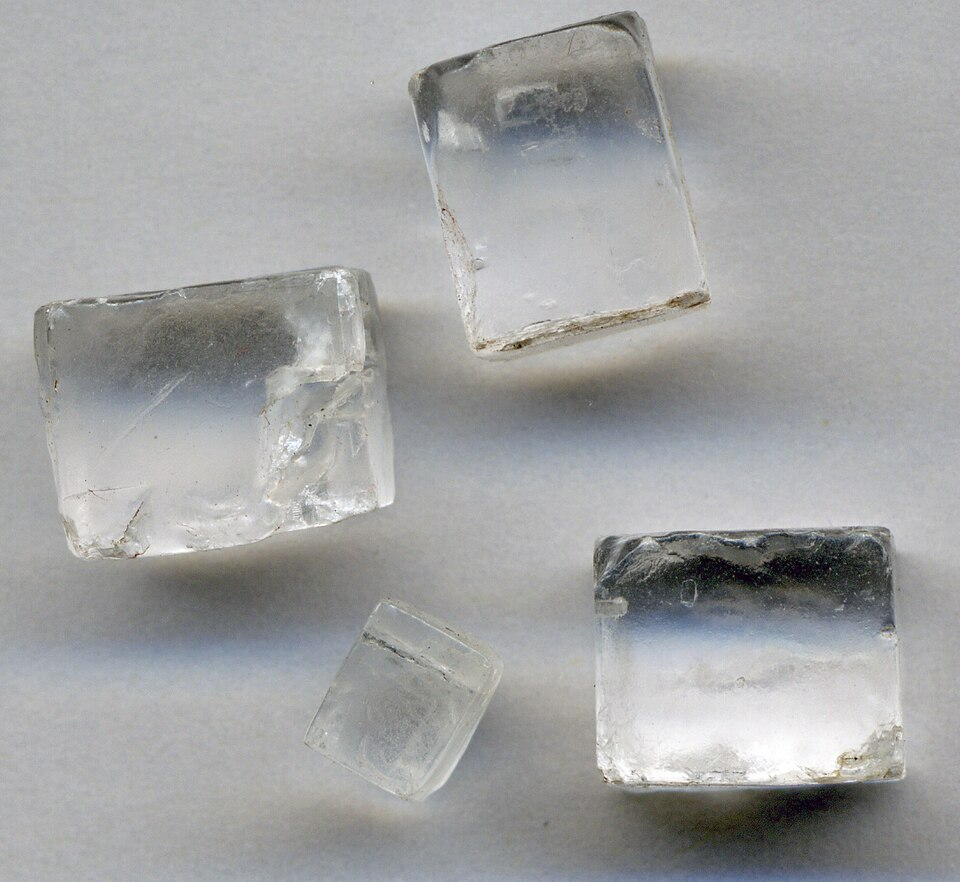
\includegraphics[width=\linewidth]{images/book2/halite.jpg}

{\small हैलाइट (सैंधव लवण) के \omterm{def:b1:crystals-metals:crystal}{क्रिस्टल}। छायाचित्र: जेम्स सेंट जॉन, CC BY 2.0।}
\end{minipage}\hfill
\begin{minipage}[b]{0.31\linewidth}\centering
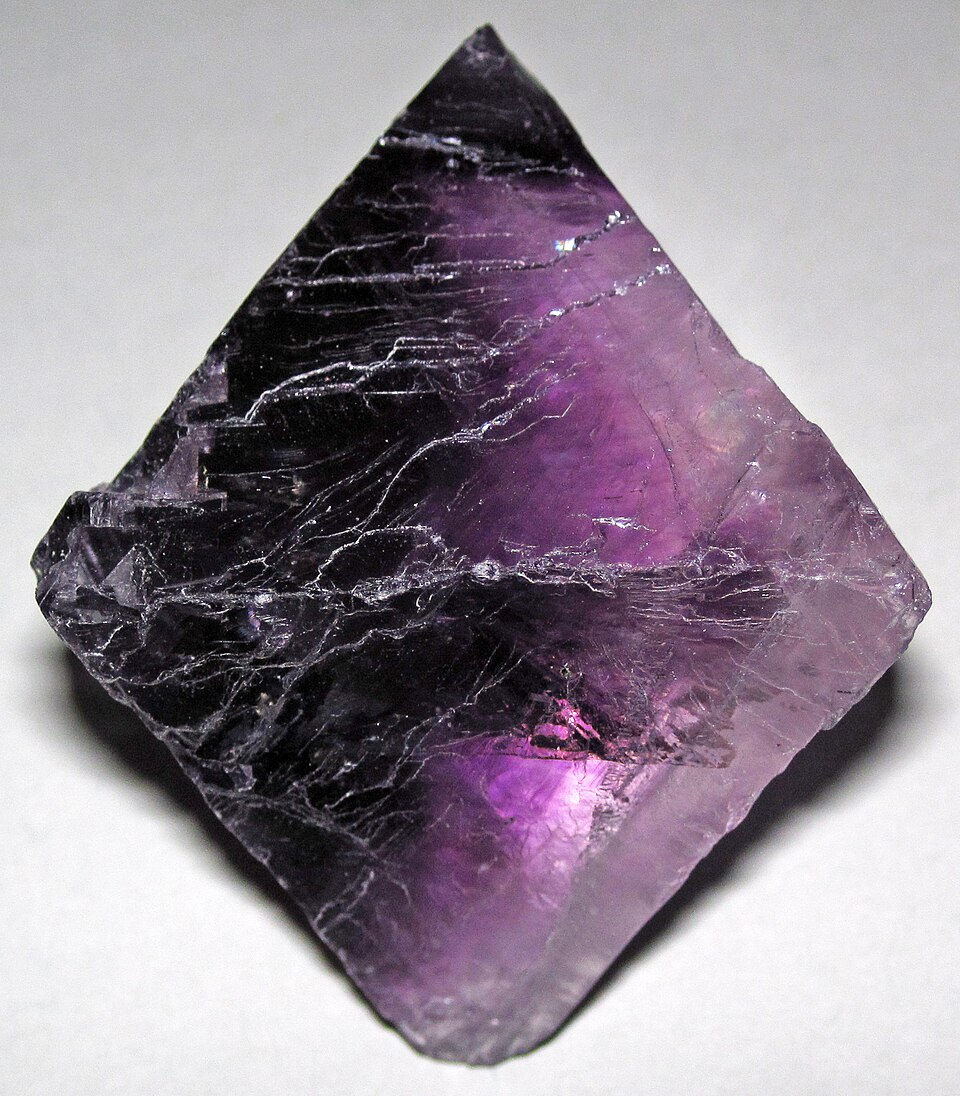
\includegraphics[width=0.85\linewidth]{images/book2/fluorite.jpg}

{\small फ़्लुओराइट, \ce{CaF2}। छायाचित्र: जेम्स सेंट जॉन, CC BY 2.0।}
\end{minipage}\hfill
\begin{minipage}[b]{0.31\linewidth}\centering
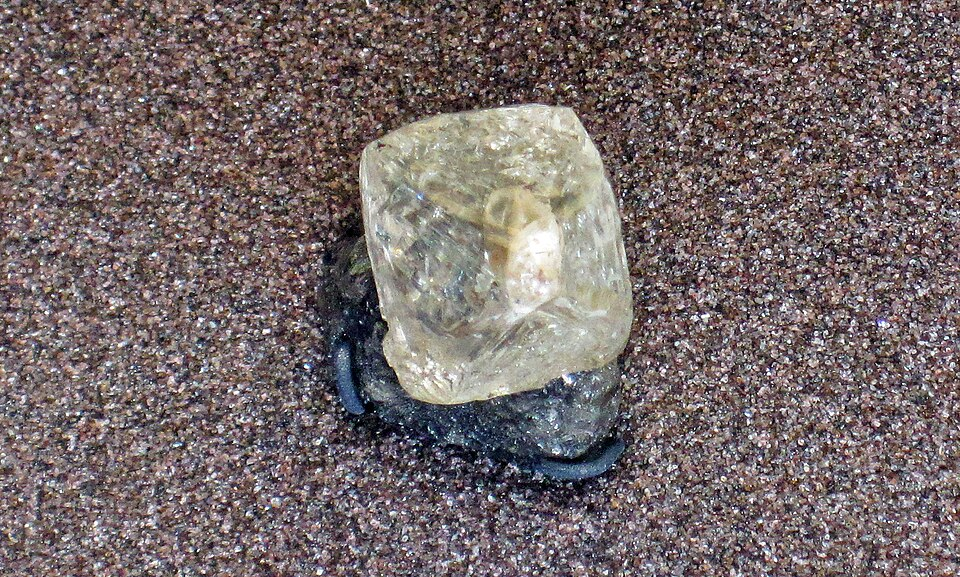
\includegraphics[width=\linewidth]{images/book2/diamond.jpg}

{\small हीरे का एक अनगढ़ अष्टफलक। छायाचित्र: जेम्स सेंट जॉन, CC BY 2.0।}
\end{minipage}
\end{omfigure}

\begin{proposition}[ज़िंक-ब्लेंड और फ़्लुओराइट प्रकार]\label{prop:b1:crystals-ionic-covalent:zns-caf2}
\omterm{def:b1:crystals-ionic-covalent:structure-type}{ज़िंक-ब्लेंड प्रकार} में $Z = 4$, हर आयन दूसरे प्रकार के चार आयनों से
चतुष्फलक के कोनों पर घिरा होता है, और आयन मुख्य विकर्ण के एक-चौथाई
के अनुदिश छूते हैं: $a\sqrt3/4 = r_+ + r_-$। \omterm{def:b1:crystals-ionic-covalent:structure-type}{फ़्लुओराइट
प्रकार} में $Z = 4$ \ce{CaF2} इकाइयाँ, हर धनायन के 8 ऋणायन पड़ोसी (एक घन),
हर ऋणायन के 4 धनायन पड़ोसी (एक चतुष्फलक), और फिर से $a\sqrt3/4 =
r_+ + r_-$।
\end{proposition}

\begin{proof}
ज़िंक ब्लेंड: FCC \omterm{def:b1:crystals-metals:lattice}{जालक} पर 4 ऋणायन और 8 \omterm{def:b1:crystals-metals:site}{चतुष्फलकीय स्थलों} में से आधे में
4 धनायन। $(\frac a4,\frac a4,\frac a4)$ पर स्थित \omterm{def:b1:crystals-metals:site}{चतुष्फलकीय स्थल}
अपने चार ऋणायनों से $\frac{a\sqrt3}{4}$ दूर है। फ़्लुओराइट: 4 धनायन और
सभी \omterm{def:b1:crystals-metals:site}{चतुष्फलकीय स्थलों} में 8 ऋणायन, अनुपात $1:2$। कोष्ठिका के भीतर के 8 ऋणायन
कोर $a/2$ वाला घन बनाते हैं, और ऋणायनों के ऐसे घनों में से हर दूसरे घन के
केंद्र पर एक धनायन होता है; किसी ऋणायन के 4 धनायन
पड़ोसी $\frac{a\sqrt3}{4}$ पर होते हैं।
\end{proof}

\begin{omfigure}
\tdplotsetmaincoords{60}{100}
\begin{tikzpicture}[tdplot_main_coords, font=\small]
  \pic {omcubeo={3}};
  \begin{scope}[on background layer]
    \draw[black!45, line width=1.2pt] (0.75,0.75,2.25) -- (0,0,3) (0.75,0.75,2.25) -- (0,1.5,1.5) (0.75,0.75,2.25) -- (1.5,0,1.5) (0.75,0.75,2.25) -- (1.5,1.5,3) (0.75,2.25,0.75) -- (0,1.5,1.5) (0.75,2.25,0.75) -- (0,3,0) (0.75,2.25,0.75) -- (1.5,1.5,0) (0.75,2.25,0.75) -- (1.5,3,1.5) (2.25,0.75,0.75) -- (1.5,0,1.5) (2.25,0.75,0.75) -- (1.5,1.5,0) (2.25,0.75,0.75) -- (3,0,0) (2.25,0.75,0.75) -- (3,1.5,1.5) (2.25,2.25,2.25) -- (1.5,1.5,3) (2.25,2.25,2.25) -- (1.5,3,1.5) (2.25,2.25,2.25) -- (3,1.5,1.5) (2.25,2.25,2.25) -- (3,3,3);
  \end{scope}
    \node[aX={yellow!75!orange}{6mm}] at (0,0,0) {};
  \node[aX={yellow!75!orange}{6mm}] at (0,3,0) {};
  \node[aX={yellow!75!orange}{6mm}] at (0,1.5,1.5) {};
  \node[aX={gray!60}{3.6mm}] at (0.75,2.25,0.75) {};
  \node[aX={yellow!75!orange}{6mm}] at (0,0,3) {};
  \node[aX={yellow!75!orange}{6mm}] at (1.5,1.5,0) {};
  \node[aX={gray!60}{3.6mm}] at (0.75,0.75,2.25) {};
  \node[aX={yellow!75!orange}{6mm}] at (0,3,3) {};
  \node[aX={yellow!75!orange}{6mm}] at (1.5,0,1.5) {};
  \node[aX={gray!60}{3.6mm}] at (2.25,0.75,0.75) {};
  \node[aX={yellow!75!orange}{6mm}] at (1.5,3,1.5) {};
  \node[aX={yellow!75!orange}{6mm}] at (3,0,0) {};
  \node[aX={yellow!75!orange}{6mm}] at (1.5,1.5,3) {};
  \node[aX={yellow!75!orange}{6mm}] at (3,3,0) {};
  \node[aX={gray!60}{3.6mm}] at (2.25,2.25,2.25) {};
  \node[aX={yellow!75!orange}{6mm}] at (3,1.5,1.5) {};
  \node[aX={yellow!75!orange}{6mm}] at (3,0,3) {};
  \node[aX={yellow!75!orange}{6mm}] at (3,3,3) {};
  \node at (1.5,1.5,-1.75) {\ce{ZnS} (ज़िंक ब्लेंड)};
\end{tikzpicture}
\hspace{1cm}
\begin{tikzpicture}[tdplot_main_coords, font=\small]
  \pic {omcubeo={3}};
    \node[aX={green!35!gray}{4.4mm}] at (0,0,0) {};
  \node[aX={green!35!gray}{4.4mm}] at (0,3,0) {};
  \node[aX={green!35!gray}{4.4mm}] at (0,1.5,1.5) {};
  \node[aX={green!45!yellow}{5.0mm}] at (0.75,0.75,0.75) {};
  \node[aX={green!45!yellow}{5.0mm}] at (0.75,2.25,0.75) {};
  \node[aX={green!35!gray}{4.4mm}] at (0,0,3) {};
  \node[aX={green!35!gray}{4.4mm}] at (1.5,1.5,0) {};
  \node[aX={green!45!yellow}{5.0mm}] at (0.75,0.75,2.25) {};
  \node[aX={green!35!gray}{4.4mm}] at (0,3,3) {};
  \node[aX={green!35!gray}{4.4mm}] at (1.5,0,1.5) {};
  \node[aX={green!45!yellow}{5.0mm}] at (0.75,2.25,2.25) {};
  \node[aX={green!45!yellow}{5.0mm}] at (2.25,0.75,0.75) {};
  \node[aX={green!35!gray}{4.4mm}] at (1.5,3,1.5) {};
  \node[aX={green!35!gray}{4.4mm}] at (3,0,0) {};
  \node[aX={green!45!yellow}{5.0mm}] at (2.25,2.25,0.75) {};
  \node[aX={green!35!gray}{4.4mm}] at (1.5,1.5,3) {};
  \node[aX={green!35!gray}{4.4mm}] at (3,3,0) {};
  \node[aX={green!45!yellow}{5.0mm}] at (2.25,0.75,2.25) {};
  \node[aX={green!45!yellow}{5.0mm}] at (2.25,2.25,2.25) {};
  \node[aX={green!35!gray}{4.4mm}] at (3,1.5,1.5) {};
  \node[aX={green!35!gray}{4.4mm}] at (3,0,3) {};
  \node[aX={green!35!gray}{4.4mm}] at (3,3,3) {};
  \node at (1.5,1.5,-1.75) {\ce{CaF2} (फ़्लुओराइट)};
\end{tikzpicture}

{\small बाएँ: ज़िंक ब्लेंड, \ce{S^{2-}} (पीला) FCC \omterm{def:b1:crystals-metals:lattice}{जालक} पर और
\ce{Zn^{2+}} (धूसर) एकांतर \omterm{def:b1:crystals-metals:site}{चतुष्फलकीय स्थलों} में, हर एक अपने
चार पड़ोसियों से जुड़ा। दाएँ: फ़्लुओराइट, \ce{Ca^{2+}} (धूसर-हरा) FCC
\omterm{def:b1:crystals-metals:lattice}{जालक} पर और \ce{F-} (हल्का हरा) सभी आठ \omterm{def:b1:crystals-metals:site}{चतुष्फलकीय स्थलों} में।}
\end{omfigure}

\begin{example}[ज़िंक ब्लेंड और फ़्लुओराइट]\label{ex:b1:crystals-ionic-covalent:zns}
ज़िंक ब्लेंड के लिए $a = \qty{540.9}{pm}$: $r_+ + r_- = a\sqrt3/4 =
\qty{234.2}{pm}$ (शैनन: $60 + 184 = \qty{244}{pm}$, क्योंकि सल्फ़ाइड की त्रिज्या
केवल छह पड़ोसियों के लिए सारणीबद्ध है), और $x = 60/184 = 0.33$,
चतुष्फलकीय परास में। फ़्लुओराइट के लिए $a = \qty{546.3}{pm}$: $r_+ + r_- =
\qty{236.6}{pm}$ (शैनन $112 + 131 = \qty{243}{pm}$), और $x = 0.85$:
धनायन 8 ऋणायनों के घन में बैठता है, जैसा नियम माँगता है।
% ledger: lat:ZnS, rion:Zn2+IV, rion:S2-VI, lat:CaF2, rion:Ca2+VIII,
% rion:F-IV
\end{example}

\begin{method}[संरचना का पूर्वानुमान]\label{met:b1:crystals-ionic-covalent:predict}
किसी आयनिक यौगिक \ce{MX} या \ce{MX2} की संरचना का पूर्वानुमान लगाने के लिए:
\begin{enumerate}
  \item सारणीबद्ध त्रिज्याओं से (अपेक्षित
        उपसहसंयोजन के लिए) $x = r_+/r_-$ परिकलित कीजिए;
  \item त्रिज्या-अनुपात नियम से धनायन की उपसहसंयोजन पढ़िए;
  \item वह प्रकार चुनिए जिसमें यह उपसहसंयोजन और सही सूत्र हो:
        8 के साथ \ce{MX}: \ce{CsCl}; 6 के साथ: \ce{NaCl}; 4 के साथ: ज़िंक ब्लेंड;
        8 के साथ \ce{MX2}: फ़्लुओराइट;
  \item मापे गए \omterm{def:b1:crystals-metals:lattice}{जालक प्राचल} से जाँचिए; याद रखिए कि
        ध्रुवणीय आयन (\ce{S^{2-}}, \ce{I-}) और छोटे, आवेशित धनायन
        आंशिक रूप से \omterm{def:b1:lewis-resonance-vsepr:lewis}{सहसंयोजी आबंध} देते हैं, जिनके लिए नियम विफल रहता है।
\end{enumerate}
\end{method}

\section{सहसंयोजी क्रिस्टल}

\begin{definition}[सहसंयोजी क्रिस्टल]\label{def:b1:crystals-ionic-covalent:covalent-crystal}
\emph{सहसंयोजी क्रिस्टल}\index{सहसंयोजी क्रिस्टल} (या जालिका ठोस) वह
\omterm{def:b1:crystals-metals:crystal}{क्रिस्टल} है जिसमें सभी परमाणु \omterm{def:b1:lewis-resonance-vsepr:lewis}{सहसंयोजी आबंधों} से जुड़कर एक
विशाल अणु बनाते हैं: हीरा, सिलिकॉन, क्वार्ट्ज़ \ce{SiO2}। ग्रेफ़ाइट जैसे परतदार
सहसंयोजी \omterm{def:b1:crystals-metals:crystal}{क्रिस्टल} में सहसंयोजी जालिका केवल
तलों में फैली होती है, जिन्हें \omterm{def:b1:intermolecular-forces-solvents:vdw}{वान्डरवाल्स अन्योन्यक्रियाएँ} एक-दूसरे से जोड़े रखती हैं।
\end{definition}

\begin{proposition}[हीरे की संरचना]\label{prop:b1:crystals-ionic-covalent:diamond}
हीरे में कार्बन परमाणु FCC \omterm{def:b1:crystals-metals:lattice}{जालक} और उसके आधे
\omterm{def:b1:crystals-metals:site}{चतुष्फलकीय स्थलों} पर होते हैं, ज़िंक ब्लेंड के दोनों प्रकार के आयनों की तरह: $Z = 8$, हर
कार्बन चतुष्फलक के कोनों पर स्थित चार अन्य कार्बनों से
दूरी $a\sqrt3/4$ पर आबंधित। स्पर्श करते गोलों के लिए \omterm{def:b1:crystals-metals:compactness}{संहतता} है
\[
  C = \frac{\pi\sqrt3}{16} \approx 0.34 .
\]
\end{proposition}

\begin{proof}
$Z = 4 + 4 = 8$। पड़ोसी परमाणु छूते हैं: $2R = a\sqrt3/4$, इसलिए $a =
8R/\sqrt3$ और $C = 8 \cdot \frac43\pi R^3/a^3 = \frac{32}{3}\pi R^3 \cdot
\frac{3\sqrt3}{512 R^3} = \frac{\pi\sqrt3}{16}$।
\end{proof}

\begin{omfigure}
\tdplotsetmaincoords{60}{100}
\begin{tikzpicture}[tdplot_main_coords, font=\small]
  \pic {omcubeo={3}};
  \begin{scope}[on background layer]
    \draw[black!55, line width=1.4pt] (0.75,0.75,2.25) -- (0,0,3) (0.75,0.75,2.25) -- (0,1.5,1.5) (0.75,0.75,2.25) -- (1.5,0,1.5) (0.75,0.75,2.25) -- (1.5,1.5,3) (0.75,2.25,0.75) -- (0,1.5,1.5) (0.75,2.25,0.75) -- (0,3,0) (0.75,2.25,0.75) -- (1.5,1.5,0) (0.75,2.25,0.75) -- (1.5,3,1.5) (2.25,0.75,0.75) -- (1.5,0,1.5) (2.25,0.75,0.75) -- (1.5,1.5,0) (2.25,0.75,0.75) -- (3,0,0) (2.25,0.75,0.75) -- (3,1.5,1.5) (2.25,2.25,2.25) -- (1.5,1.5,3) (2.25,2.25,2.25) -- (1.5,3,1.5) (2.25,2.25,2.25) -- (3,1.5,1.5) (2.25,2.25,2.25) -- (3,3,3);
  \end{scope}
  \node[aX={black!65}{3.6mm}] at (0,0,0) {};
  \node[aX={black!65}{3.6mm}] at (0,3,0) {};
  \node[aX={black!65}{3.6mm}] at (0,1.5,1.5) {};
  \node[aX={black!65}{3.6mm}] at (0.75,2.25,0.75) {};
  \node[aX={black!65}{3.6mm}] at (0,0,3) {};
  \node[aX={black!65}{3.6mm}] at (1.5,1.5,0) {};
  \node[aX={black!65}{3.6mm}] at (0.75,0.75,2.25) {};
  \node[aX={black!65}{3.6mm}] at (0,3,3) {};
  \node[aX={black!65}{3.6mm}] at (1.5,0,1.5) {};
  \node[aX={black!65}{3.6mm}] at (2.25,0.75,0.75) {};
  \node[aX={black!65}{3.6mm}] at (1.5,3,1.5) {};
  \node[aX={black!65}{3.6mm}] at (3,0,0) {};
  \node[aX={black!65}{3.6mm}] at (1.5,1.5,3) {};
  \node[aX={black!65}{3.6mm}] at (3,3,0) {};
  \node[aX={black!65}{3.6mm}] at (2.25,2.25,2.25) {};
  \node[aX={black!65}{3.6mm}] at (3,1.5,1.5) {};
  \node[aX={black!65}{3.6mm}] at (3,0,3) {};
  \node[aX={black!65}{3.6mm}] at (3,3,3) {};
  \node at (1.5,1.5,-1.75) {हीरा};
\end{tikzpicture}
\hspace{0.8cm}
\begin{tikzpicture}[font=\small, y={(0cm,0.45cm)}, z={(0cm,1cm)}, x={(1cm,0cm)}]
  % two honeycomb layers seen in perspective, ABAB stacking
  \foreach \zz/\dy/\col in {0/0/black!40, 1.7/0.82/black!80} {
    \foreach \i in {0,1,2} \foreach \j in {0,1} {
      \pgfmathsetmacro\cx{1.42*\i+0.71*\j}
      \pgfmathsetmacro\cy{1.23*\j+\dy}
      \foreach \k in {0,60,...,300} {
        \pgfmathsetmacro\ka{\k+60}
        \draw[\col, line width=1pt] ({\cx+0.82*cos(\k+30)},{\cy+0.82*sin(\k+30)},\zz)
          -- ({\cx+0.82*cos(\ka+30)},{\cy+0.82*sin(\ka+30)},\zz);
      }
    }
  }
  \draw[<->, omThm] (5.6,0.9,0) -- (5.6,0.9,1.7) node[midway, right] {\qty{335}{pm}};
  \node at (2.4,-1.6,0) {ग्रेफ़ाइट};
\end{tikzpicture}

{\small बाएँ: हीरे की कोष्ठिका, हर कार्बन चतुष्फलक में चार अन्य कार्बनों से
आबंधित। दाएँ: ग्रेफ़ाइट, षट्भुजों की परतें (परत के भीतर C--C \qty{141.8}{pm})
एक-दूसरे से \qty{334.8}{pm} दूर जमी हुई, लंदन बलों से जुड़ी हुई;
परतें ABAB क्रम में एकांतर हैं।}
% ledger: lat:C-graphite.a, lat:C-graphite.c (C-C = a/sqrt3; interlayer = c/2)
\end{omfigure}

\begin{example}[हीरा, सिलिकॉन, ग्रेफ़ाइट]\label{ex:b1:crystals-ionic-covalent:carbon}
हीरे के लिए $a = \qty{356.7}{pm}$: \ce{C-C} $= a\sqrt3/4 =
\qty{154.5}{pm}$, जो एथेन का एकल आबंध है, और $\rho =
\qty{3.52}{g/cm^3}$। उसी संरचना वाले सिलिकॉन के लिए, $a =
\qty{543.1}{pm}$ के साथ, \ce{Si-Si} $= \qty{235.2}{pm}$ और $\rho =
\qty{2.33}{g/cm^3}$ (मापा गया 2.33)। ग्रेफ़ाइट में हर कार्बन एक तल में
तीन अन्य कार्बनों से \qty{141.8}{pm} पर आबंधित है, जो एक और दो के बीच की आबंध कोटि
है (पूरी परत पर अनुनाद), जबकि परतें
\qty{334.8}{pm} दूर हैं। हीरा, तीनों विमाओं में दृढ़, सबसे कठोर
प्राकृतिक पदार्थ और एक विद्युतरोधी है; ग्रेफ़ाइट अपनी परतों के बीच विदलित होता है,
जो आसानी से फिसलती हैं, और अपने विस्थानीकृत $\pi$ इलेक्ट्रॉनों के कारण उनके भीतर
विद्युत का चालन करता है।
% ledger: lat:C-diamond, lat:Si, rho:Si, lat:C-graphite.a, lat:C-graphite.c,
% geo:C2H6.rCC
\end{example}

\begin{omfigure}
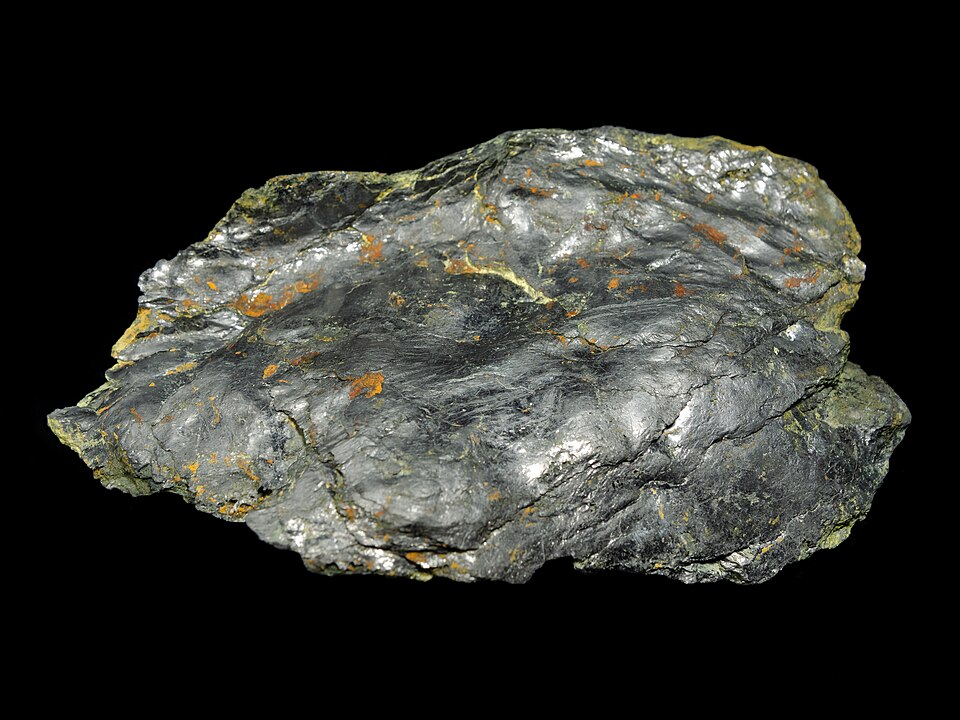
\includegraphics[width=0.36\linewidth]{images/book2/graphite.jpg}

{\small प्राकृतिक ग्रेफ़ाइट का एक नमूना, अपनी धात्विक चमक के साथ। छायाचित्र:
ज़बिनेक बुरिवाल, CC BY-SA 4.0।}
\end{omfigure}

\section{आण्विक क्रिस्टल}

\begin{definition}[आण्विक क्रिस्टल]\label{def:b1:crystals-ionic-covalent:molecular-crystal}
\emph{आण्विक क्रिस्टल}\index{आण्विक क्रिस्टल} अणुओं का ऐसा \omterm{def:b1:crystals-metals:crystal}{क्रिस्टल} है
जिन्हें अंतराआण्विक बल --- \omterm{def:b1:intermolecular-forces-solvents:vdw}{वान्डरवाल्स
अन्योन्यक्रियाएँ} और, जहाँ संभव हो, \omterm{def:b1:intermolecular-forces-solvents:hbond}{हाइड्रोजन आबंध} --- जोड़े रखते हैं, जबकि हर अणु
अपने \omterm{def:b1:lewis-resonance-vsepr:lewis}{सहसंयोजी आबंध} बनाए रखता है: डाइआयोडीन, शुष्क बर्फ़ \ce{CO2(s)}, बर्फ़, शक्कर।
\end{definition}

\begin{proposition}[आण्विक क्रिस्टलों के गुण]\label{prop:b1:crystals-ionic-covalent:molecular}
\omterm{def:b1:crystals-ionic-covalent:molecular-crystal}{आण्विक क्रिस्टल} नरम होते हैं और कम ताप पर पिघलते या ऊर्ध्वपातित होते हैं,
क्योंकि केवल दुर्बल अंतराआण्विक बल टूटते हैं; वे चालन नहीं करते।
\end{proposition}
\admitted

\begin{example}[बर्फ़]\label{ex:b1:crystals-ionic-covalent:ice}
साधारण बर्फ़ में हर पानी का अणु चतुष्फलक के कोनों पर स्थित चार अन्य अणुओं से
हाइड्रोजन-आबंधित होता है: दो से अपने हाइड्रोजनों द्वारा और दो से अपने
\omterm{def:b1:lewis-resonance-vsepr:lewis}{एकाकी युग्मों} द्वारा। यह खुली, षट्कोणीय जालिका, जो \omterm{def:b1:intermolecular-forces-solvents:hbond}{हाइड्रोजन आबंधों} की दिशाओं
द्वारा थोपी जाती है, बहुत ख़ाली जगह छोड़ती है: बर्फ़ द्रव
पानी से कम घनी है, जिसमें जालिका आंशिक रूप से टूटी होती है और अणु
पास आ जाते हैं। जालिका की षट्कोणीय सममिति हिम-क्रिस्टलों की षट्गुण आकृति
में दिखती है।
\end{example}

\begin{omfigure}
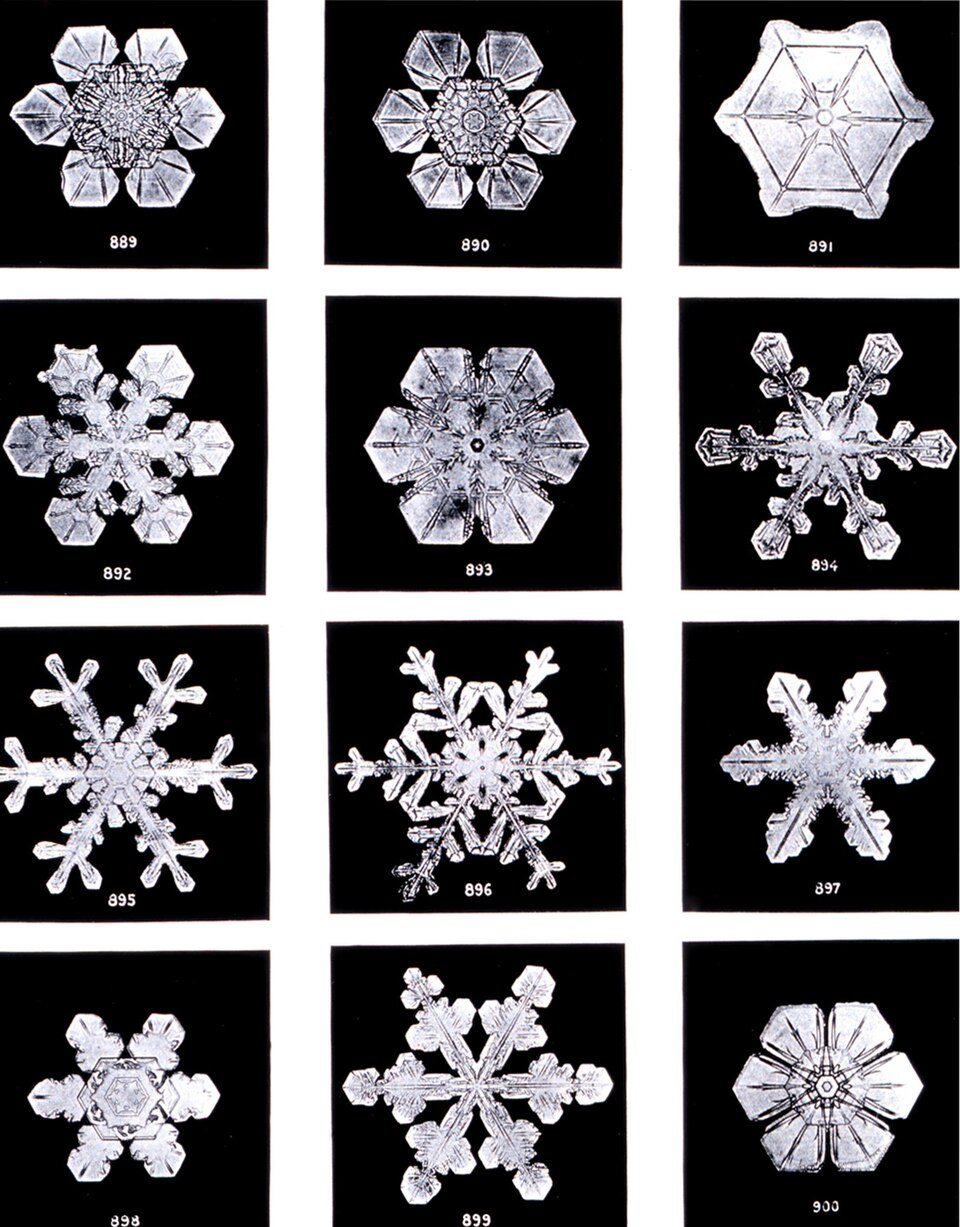
\includegraphics[width=0.38\linewidth]{images/book2/bentley-snowflakes.jpg}

{\small विल्सन बेंटली द्वारा लगभग 1902 में खींचे गए हिम-क्रिस्टल: हर एक
में षट्गुण सममिति है, जो बर्फ़ में \omterm{def:b1:intermolecular-forces-solvents:hbond}{हाइड्रोजन आबंधों} की षट्कोणीय जालिका का
चिह्न है। सार्वजनिक अधिकार-क्षेत्र।}
\end{omfigure}

\section{चार प्रकार के ठोसों की तुलना}

\begin{center}
\small
\begin{tabular}{lllll}
\hline
ठोस & कण & संसंजन & गुण & उदाहरण \\
\hline
धात्विक & धनायन, इलेक्ट्रॉन & \omterm{def:b1:crystals-metals:metallic-bond}{धात्विक आबंध} & चालक, तन्य & \ce{Cu}, \ce{Fe}, \ce{Na} \\
आयनिक & धनायन, ऋणायन & स्थिरवैद्युत & कठोर, भंगुर, विद्युतरोधी & \ce{NaCl}, \ce{CaF2} \\
सहसंयोजी & परमाणु & \omterm{def:b1:lewis-resonance-vsepr:lewis}{सहसंयोजी आबंध} & अति कठोर, उच्च गलनांक & हीरा, \ce{SiO2} \\
आण्विक & अणु & वान्डरवाल्स, H आबंध & नरम, निम्न गलनांक & \ce{I2}, बर्फ़ \\
\hline
\end{tabular}
\end{center}

\begin{remark}[एक सातत्य]\label{rem:b1:crystals-ionic-covalent:continuum}
ये वर्ग आदर्शीकरण हैं। ज़िंक सल्फ़ाइड के आबंध आंशिक रूप से आयनिक,
आंशिक रूप से सहसंयोजी हैं, इसीलिए उसकी सल्फ़ाइड--ज़िंक दूरी
\omterm{def:b1:periodicity:radius}{आयनिक त्रिज्याओं} के योग से कम है; ग्रेफ़ाइट अपनी परतों में सहसंयोजी है और
उनके बीच आण्विक। \omterm{def:b1:periodicity:electronegativity}{विद्युत-ऋणात्मकता} का अंतर
(\cref{prop:b1:periodicity:en-trend}) मार्गदर्शक है: वह जितना बड़ा, ठोस
उतना अधिक आयनिक।
\end{remark}

\section{अभ्यास}

\begin{exercise}[$\star$]\label{exo:b1:crystals-ionic-covalent:1}
सैंधव-लवण कोष्ठिका में धनायनों और ऋणायनों को गिनिए, हर एक की
उपसहसंयोजन बताइए, और जाँचिए कि सूत्र \ce{NaCl} का पालन होता है।
\end{exercise}

\begin{exercise}[$\star$]\label{exo:b1:crystals-ionic-covalent:2}
सीज़ियम क्लोराइड के लिए $a = \qty{412.3}{pm}$। सबसे छोटी
\ce{Cs-Cl} दूरी और प्रति कोष्ठिका सूत्र इकाइयों की संख्या परिकलित कीजिए।
\end{exercise}

\begin{exercise}[$\star$]\label{exo:b1:crystals-ionic-covalent:3}
त्रिज्याओं $r(\ce{Na+}) = \qty{102}{pm}$ और $r(\ce{Cl-}) =
\qty{181}{pm}$ से \ce{NaCl} का \omterm{def:b1:crystals-ionic-covalent:radius-ratio}{त्रिज्या अनुपात} परिकलित कीजिए और
धनायन की उपसहसंयोजन का पूर्वानुमान लगाइए।
\end{exercise}

\begin{exercise}[$\star$]\label{exo:b1:crystals-ionic-covalent:4}
धात्विक, आयनिक, सहसंयोजी या आण्विक में वर्गीकृत कीजिए: कॉपर, सोडियम
क्लोराइड, हीरा, डाइआयोडीन, क्वार्ट्ज़ \ce{SiO2}, बर्फ़, कैल्सियम फ़्लुओराइड।
\end{exercise}

\begin{exercise}[$\star\star$]\label{exo:b1:crystals-ionic-covalent:5}
सिद्ध कीजिए कि सैंधव-लवण संरचना के लिए $r_+/r_- \ge \sqrt2 - 1$ आवश्यक है।
\end{exercise}

\begin{exercise}[$\star\star$]\label{exo:b1:crystals-ionic-covalent:6}
$a = \qty{564.1}{pm}$ से सोडियम क्लोराइड का घनत्व परिकलित कीजिए
($M(\ce{NaCl}) = \qty{58.44}{g/mol}$) और
\qty{2.17}{g/cm^3} से तुलना कीजिए।
\end{exercise}

\begin{exercise}[$\star\star$]\label{exo:b1:crystals-ionic-covalent:7}
सीज़ियम क्लोराइड का घनत्व परिकलित कीजिए ($M = \qty{168.36}{g/mol}$,
$a = \qty{412.3}{pm}$) और मापे गए \qty{3.99}{g/cm^3} से तुलना कीजिए।
% ledger: rho:CsCl
\end{exercise}

\begin{exercise}[$\star\star$]\label{exo:b1:crystals-ionic-covalent:8}
ज़िंक ब्लेंड ($a = \qty{540.9}{pm}$, $M = \qty{97.44}{g/mol}$) के लिए
\ce{Zn-S} दूरी और घनत्व परिकलित कीजिए, और मापे गए
\qty{4.04}{g/cm^3} से तुलना कीजिए।
% ledger: rho:ZnS
\end{exercise}

\begin{exercise}[$\star\star$]\label{exo:b1:crystals-ionic-covalent:9}
ग्रेफ़ाइट की षट्कोणीय कोष्ठिका में $a = \qty{245.6}{pm}$ और
$c = \qty{669.6}{pm}$ हैं, और उसमें 4 परमाणु हैं। परत में \ce{C-C} दूरी
($a/\sqrt3$), परतों के बीच की दूरी ($c/2$) और
घनत्व परिकलित कीजिए। ग्रेफ़ाइट हीरे से कम घना क्यों है?
\end{exercise}

\begin{exercise}[$\star\star\star$]\label{exo:b1:crystals-ionic-covalent:10}
सिद्ध कीजिए कि हीरे की \omterm{def:b1:crystals-metals:compactness}{संहतता} $\pi\sqrt3/16$ है, और समझाइए कि
सबसे कठोर पदार्थ सबसे कम संहत पदार्थों में से एक क्यों है।
\end{exercise}

\begin{exercise}[$\star\star\star$]\label{exo:b1:crystals-ionic-covalent:11}
सिलिकॉन की संरचना हीरे वाली है, $a = \qty{543.1}{pm}$ के साथ।
\ce{Si-Si} आबंध लंबाई, सिलिकॉन की \omterm{def:b1:periodicity:radius}{सहसंयोजी त्रिज्या} और
घनत्व ($M = \qty{28.09}{g/mol}$) परिकलित कीजिए; \qty{2.33}{g/cm^3} से तुलना कीजिए।
\end{exercise}

\begin{exercise}[$\star\star\star$]\label{exo:b1:crystals-ionic-covalent:12}
रुबिडियम क्लोराइड के लिए $r(\ce{Rb+}) = \qty{152}{pm}$ (छह पड़ोसी) और
$r(\ce{Cl-}) = \qty{181}{pm}$। त्रिज्या-अनुपात नियम किस संरचना का
पूर्वानुमान देता है? सामान्य परिस्थितियों में यह \omterm{def:b1:crystals-ionic-covalent:structure-type}{सैंधव-लवण प्रकार} का है,
$a = \qty{658.1}{pm}$ के साथ: \ce{Rb-Cl} दूरी जाँचिए, और सुझाइए कि
नियम यहाँ क्यों विफल होता है।
% ledger: rion:Rb+VI, rion:Cl-VI, lat:RbCl
\end{exercise}

\section{समस्या: फ़्लुओराइट, खनिज और लेंस}

\begin{problem}[{सप्ताहांत समस्या --- फ़्लुओराइट की कोष्ठिका, उसका \omterm{def:b1:crystals-ionic-covalent:radius-ratio}{त्रिज्या अनुपात},
दो संबंधी (\ce{Li2O} और हीरा), और कोष्ठिका से परिकलित
फ़्लुओराइट का घनत्व}]
\label{pb:b1:crystals-ionic-covalent:1}
फ़्लुओराइट, \ce{CaF2}, एक खनिज है; बड़े पारदर्शी \omterm{def:b1:crystals-metals:crystal}{क्रिस्टलों} के रूप में उगाया जाए तो उससे
ऐसे लेंस बनते हैं जो पराबैंगनी प्रकाश को पार जाने देते हैं। इसकी कोष्ठिका घनीय है, $a =
\qty{546.3}{pm}$; \ce{Ca^{2+}} FCC \omterm{def:b1:crystals-metals:lattice}{जालक} पर, \ce{F-}
\omterm{def:b1:crystals-metals:site}{चतुष्फलकीय स्थलों} में। त्रिज्याएँ: $r(\ce{Ca^{2+}}) = \qty{112}{pm}$ (आठ
पड़ोसी), $r(\ce{F-}) = \qty{131}{pm}$ (चार पड़ोसी)। मोलर द्रव्यमान
(g/mol): \ce{Ca} 40.08, \ce{F} 19.00, \ce{Li} 6.94, \ce{O} 16.00, \ce{C}
12.01, \ce{Si} 28.09; $N_A = \qty{6.022e23}{mol^{-1}}$।
% ledger: lat:CaF2, rion:Ca2+VIII, rion:F-IV, aw:Ca, aw:F, aw:Li, aw:O,
% aw:C, aw:Si, const:NA

\medskip
\noindent\textbf{भाग I --- कोष्ठिका।}
\begin{enumerate}
  \item कोष्ठिका में \ce{Ca^{2+}} आयनों की स्थितियाँ बताइए और उन्हें
        गिनिए।
  \item कोष्ठिका में कितने \omterm{def:b1:crystals-metals:site}{चतुष्फलकीय स्थल} हैं? इससे
        \ce{F-} आयनों की संख्या निकालिए और सूत्र की जाँच कीजिए।
  \item \ce{F-} की उपसहसंयोजन क्या है? \ce{Ca^{2+}} की?
  \item सबसे छोटी \ce{Ca-F} दूरी परिकलित कीजिए।
  \item इसकी तुलना \omterm{def:b1:periodicity:radius}{आयनिक त्रिज्याओं} के योग से कीजिए।
  \item सबसे छोटी \ce{F-F} दूरी परिकलित कीजिए और बताइए कि
        ऋणायन एक-दूसरे को छूते हैं या नहीं।
\end{enumerate}

\medskip
\noindent\textbf{भाग II --- \omterm{def:b1:crystals-ionic-covalent:radius-ratio}{त्रिज्या अनुपात}।}
\begin{enumerate}[resume]
  \item $x = r_+/r_-$ परिकलित कीजिए।
  \item त्रिज्या-अनुपात नियम धनायन की कौन-सी उपसहसंयोजन अनुमत करता है?
  \item \ce{CaF2} सीज़ियम क्लोराइड संरचना क्यों नहीं अपना सकता, यद्यपि
        उसका धनायन 8-उपसहसंयोजित है?
  \item फ़्लुओराइट का वर्णन \ce{F-} की सरल घनीय व्यवस्था के रूप में कीजिए, जिसमें
        \ce{Ca^{2+}} आधे छोटे घनों के केंद्रों में हैं।
  \item फ़्लुओराइट की \omterm{def:b1:crystals-metals:compactness}{संहतता} परिकलित कीजिए।
\end{enumerate}

\medskip
\noindent\textbf{भाग III --- दो संबंधी।}
लीथियम ऑक्साइड, \ce{Li2O}, प्रतिफ़्लुओराइट है, $a = \qty{461.9}{pm}$ के साथ;
$r(\ce{Li+}) = \qty{59}{pm}$ (चार पड़ोसी), $r(\ce{O^{2-}}) =
\qty{142}{pm}$ (आठ पड़ोसी)। हीरा: $a = \qty{356.7}{pm}$।
% ledger: lat:Li2O, rion:Li+IV, rion:O2-VIII, rho:Li2O, lat:C-diamond
\begin{enumerate}[resume]
  \item प्रतिफ़्लुओराइट कोष्ठिका में \ce{O^{2-}} और \ce{Li+} आयन
        कहाँ हैं?
  \item \ce{Li-O} दूरी परिकलित कीजिए और उसकी तुलना
        त्रिज्याओं के योग से कीजिए।
  \item \ce{Li2O} का घनत्व परिकलित कीजिए और मापे गए
        \qty{2.01}{g/cm^3} से तुलना कीजिए।
  \item किस आयनिक संरचना में स्थितियों की व्यवस्था
        हीरे जैसी ही है?
  \item हीरे की \ce{C-C} आबंध लंबाई और घनत्व परिकलित कीजिए।
  \item हीरा फ़्लुओराइट से इतना कम संहत क्यों है, यद्यपि उसके
        परमाणु उसी प्रकार की स्थितियाँ भरते हैं?
\end{enumerate}

\medskip
\noindent\textbf{भाग IV --- फ़्लुओराइट का घनत्व।}
\begin{enumerate}[resume]
  \item \ce{CaF2} का मोलर द्रव्यमान परिकलित कीजिए।
  \item एक कोष्ठिका का द्रव्यमान परिकलित कीजिए।
  \item एक कोष्ठिका का आयतन \unit{cm^3} में परिकलित कीजिए।
  \item यदि हर सौ कोष्ठिकाओं में एक \ce{F-} स्थल रिक्त हो, तो घनत्व पर
        क्या प्रभाव पड़ेगा?
  \item कोष्ठिका से फ़्लुओराइट का घनत्व परिकलित कीजिए, और उसकी तुलना
        मापे गए \qty{3.18}{g/cm^3} से कीजिए।
\end{enumerate}
% ledger: rho:CaF2
\end{problem}
